\section{Motivation}\label{sec:motivation}

\begin{figure}[t]\centering
\begin{minipage}{0.55\textwidth}
  \centering
  \lstset{style=mystyle}
\begin{lstlisting}[language=C]
int demo(int a, int b, int c){
    int r = 1;  int max = a;
    bool c1 = max < b;
    if (c1){ max = b; r = 2;  }
    bool c2 = max < c;
    if (c2){ r = 3; }
    return r;
}
\end{lstlisting}\vspace*{-3mm}
\caption{The richest one of three millionaires}
\label{fig:motivation}
\end{minipage}
\hfill
\begin{minipage}{0.4\textwidth}
  \centering
	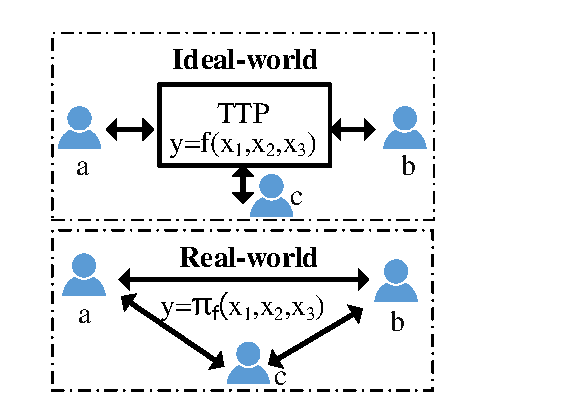
\includegraphics[scale=0.55]{img/ideal-real-v2}
     \caption{Ideal-world vs. real-world}
	\label{fig:ideal-real}
\end{minipage}
%\vspace{-2mm}
\end{figure}
%
%\begin{figure}[t]
%\centering
%\begin{subfigure}{0.5\textwidth}\centering
%\lstset{style=mystyle}
%\begin{lstlisting}[language=C]
%int demo(int a, int b, int c){
%    int r = 1;  int max = a;
%    bool c1 = max < b;
%    if (c1){ max = b; r = 2; }
%    bool c2 = max < c;
%    if (c2){ r = 3; }
%    return r;
%}
%\end{lstlisting}\vspace*{-3mm}
%\caption{The richest one of three millionaires}
%\label{fig:motivation}
%\end{subfigure}
%\quad%\vspace*{-3mm}
%\begin{subfigure}{0.4\textwidth}\centering
%    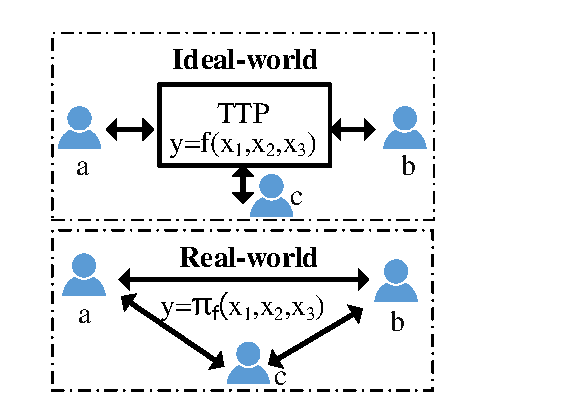
\includegraphics[scale=0.55]{img/ideal-real-v2.pdf}
%    \caption{Ideal-world vs. real-world}
%    \label{fig:ideal-real}
%\end{subfigure}
%\caption{Motivating example}
%\end{figure}

%
%\begin{figure}[t]
%\centering \lstset{style=mystyle}
%\begin{lstlisting}[language=C]
%int demo(int a, int b, int c){
%    int r = 1;  int max = a;
%    bool c1 = max < b;
%    if (c1){ max = b; r = 2; }
%    bool c2 = max < c;
%    if (c2){ r = 3; }
%    return r;
%}
%\end{lstlisting}
%\vspace*{-3mm}
%\caption{The richest one of three millionaires}
%\label{fig:motivation}
%\end{figure}
%
%\begin{figure}[t]
%    \centering
%    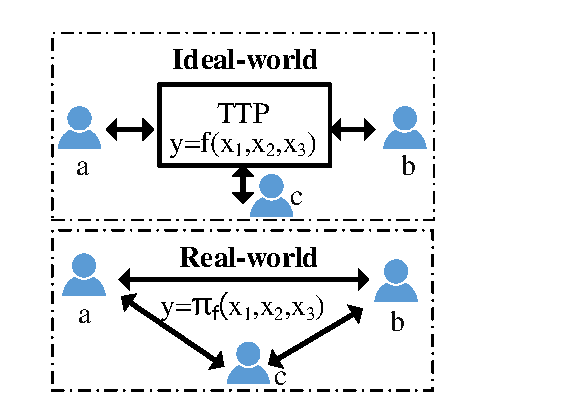
\includegraphics[scale=0.5]{img/ideal-real-v2.pdf}
%    \caption{Ideal-world vs. real-world}
%    \label{fig:ideal-real}
%\end{figure}

Fig.~\ref{fig:motivation} shows a motivating example that computes the richest among three millionaires. %Obviously, whoever executes this program  will know all the inputs   {\tt a}, {\tt b} and {\tt c}.
To preserve the privacy, the millionaires can privately send their inputs to a trusted third party (TTP)
%which computes and sends back the result,
as shown in Fig.~\ref{fig:ideal-real} (ideal-world). This reveals
the richest millionaire with the least leakage of information.
Table~\ref{tab:max3table} shows the leakage  for each result ${\tt r}=1, 2, 3$, as well as the leakage if the secret branching variables {\tt c1} and {\tt c2} are declassified (i.e., from secret to public).

\begin{table}[ht]\vspace{-7mm}
\setlength{\tabcolsep}{4mm}
\centering
\caption{Leakage from each result and declassified secret branching variables}
\label{tab:max3table}
\begin{tabular}{c|c|c|c}
\hline
\textbf{Result}  &  \textbf{Leakage of Result} &\textbf{Leakage of c1} & \textbf{Leakage of  c2} \\ \hline
${\tt r} = 1$   &${\tt a}\geq{\tt b} \wedge {\tt a}\geq{\tt c}$ & ${\tt a}\geq {\tt b}$ & ${\tt a}\geq{\tt c}$    \\ \hline
${\tt r}= 2$    & ${\tt a}<{\tt b} \wedge {\tt b}\geq {\tt c}$ &${\tt a}<{\tt b}$  & ${\tt b}\geq {\tt c}$     \\ \hline
${\tt r}= 3$    &  ${\tt c}>\max({\tt a},{\tt b})$  & ${\tt a}\geq{\tt b}\vee{\tt a}<{\tt b}$ &  ${\tt c}>\max({\tt a},{\tt b})$            \\
\hline
\end{tabular}
\vspace{-4mm}
\end{table}

To achieve the same functionality without TTP, secure multi-party computation (MPC) was proposed~\cite{Yao86,ChaumCD88,GMW,yao82,EvansKR18}. %~\cite{EvansKR18}.
%There are three fundamental MPC protocols: garbled circuits~\cite{yao82,freexor}, secret sharing~\cite{Shamir79,GMW}, and homomorphic encryption~\cite{SHE}.
One can implement the computation using an MPC protocol $\pi$  where
all the parties collaboratively compute the result over their private inputs
%following a MPC protocol
via network communications (shown in Fig.~\ref{fig:ideal-real} (real-world)).
%However, implementing the entire program in an MPC protocol is not efficient in terms of the cost of
%communication and computation.
%Therefore,

To facilitate the application of MPC, MPC frameworks, e.g., Obliv-C~\cite{ZahurE15}, MP-SPDZ~\cite{spdz20} and MPyC~\cite{MPyC20}, are proposed, which provide high-level languages
for %implementing
specifying MPC applications, as well as compilers for translating them into executable implementations.
To improve the performance, such frameworks often allow users to declare secret variables so that only
the values of secret variables are to be protected.
However, in practice, it could be highly non-trivial for non-experts to specify secret variables properly:
declaring too many secret variables degrades the performance while
declaring too less secret variables compromises security.
%As a dishonest party can observe all the intermediate computation results of the program executed by
%the dishonest party.

In this work, we propose an automated synthesis approach %for generating
%security policy which
to declare as few secret variables as possible but without compromising security.
To capture privacy, we formalize the leakage of MPC applications in the ideal-world as a set of %indistinguishable space of
private inputs. For instance, the leakage of the result ${\tt r}=1$ in the motivating example
is the set of inputs %for ${\tt a, b, c}$
such that
${\tt a}\geq{\tt b} \wedge {\tt a}\geq{\tt c}$.
We introduce the notion of security policy, which assigns each variable a security level, to bridge the language-level and protocol-level leakages, so that our approach is independent of specific MPC protocols being used.
The language-level leakage of a security policy is characterized by a set of %indistinguishable space of
private inputs with respect to not only the result but also the values of public variables
in the intermediate computations.
%A security policy should not compromise security, i.e.,
%leak more information as that in the ideal-world.


Based on the leakage characterization, we propose a type system to infer security policies,
inspired by the work for  %that for proving
the noninterference property of programs~\cite{VolpanoIS96}.
Our type system tracks both control-flow and data-flow of information from the private inputs, and infers
a security policy. For instance,
all the variables in the motivating example are inferred as secret.

Though a security policy inferred by the type system formally guarantees that the MPC application will not leak more information than that in the ideal-world, it may be too conservative.
For instance, declassifying the variable {\tt c2} in the example would not compromise security.
As shown in Table~\ref{tab:max3table}, the leakage caused by declassifying {\tt c2} can be deduced from
%is already included in
the leakage of the result. In contrast, we cannot declassify {\tt c1},
as neither ${\tt a}\geq{\tt b}$ nor ${\tt a}<{\tt b}$ can be deduced from the leakage ${\tt c}>\max({\tt a},{\tt b})$.
Once {\tt c1} is declassified, the adversary would learn
if ${\tt a}\geq{\tt b}$ or ${\tt a}<{\tt b}$.
This problem is akin to downgrading and declassification of high security levels in information-flow analysis~\cite{LiZ05}, and could be solved via self-composition~\cite{TerauchiA05,mpcleak18,YangVSGM18}
that often require users to write annotations for procedure contracts and loop invariants.
 %which reduces to the safety problem on two copies of a program
%However, it is still challenging in practice to check safety properties on two copies of a program.
%To address this issue,
In this work, for the sake of efficiency and usability for non-experts,
we propose an alternative approach based on symbolic execution~\cite{King76}.
We leverage a symbolic execution to represent a potentially infinite set of concrete executions and propose an automated approach to infer
if a secret variable can be declassified by reasoning about pairs of symbolic executions.
%\fu{Limiting the reasoning to each pair of symbolic executions could prune away
%irrelevant verification conditions and tightens the search space.}
Our approach can identify that {\tt c2} in the motivating example
can be declassified without compromising security.
The experimental results show that this approach without requiring any annotations for procedure contracts or loop invariants is effective and
the generated security policies can significantly improve
the performance of MPC applications. % when compiled into executable implementations.

%
%Participants can evaluate any function on MPC as long as they agree on it. However, not all functions are privacy-preserving.
%For example, the famous Yao's Millionaires Problem outputs the r of two millionaires without leaking any additional information about their wealth.
%%Each millionaire also knows his wealth.
%With the result of the Millionaires Problem, a millionaire learn the range of another's wealth.
%Such functions leak information from their results.
%Furthermore, a feature of these functions is that they always output symbols or indexes as the results.
%We focus on these kinds of functions and start from an example program in Fig. \ref{max3}.
%
%\lstdefinestyle{mystyle}{
%basicstyle=\ttfamily\footnotesize,
%breakatwhitespace=false,
%breaklines=true,
%captionpos=b,
%keepspaces=true,
%numbersep=5pt,
%showspaces=false,
%showstringspaces=false,
%showtabs=false,
%tabsize=2
%}
%\begin{figure}[ht]
%\centering \lstset{style=mystyle}
%\begin{lstlisting}[language=C]
%obliv char millionaire3(obliv int a, obliv int b, obliv int c){
%    obliv char r = 'a';
%    obliv int max = a;
%    obliv bool c1 = max < b;
%    obliv if (c1){
%        max = b;
%        r = 'b';
%    }
%    obliv bool c2 = max < c;
%    obliv if (c2){
%        r = 'c';
%    }
%    return r;
%}
%\end{lstlisting}
%\caption{The richest one of three millionaires \label{max3}}
%\end{figure}
%
%
%This program outputs who inputs the maximum value.
%It is an extension of Yao's Millionaires Problem.
%The \texttt{obliv \textbf{int}} in Fig. \ref{max3} declares an oblivious integer variable that represents integer typed privacy data.
%\texttt{millionaire3} function contains two if-statements, and applies oblivious control structures.
%The oblivious control structure \texttt{obliv \textbf{if}} makes participants do not know which branch is executed to keep the condition variable privacy.
%\texttt{millionaire3} has three types of output:\texttt{'a'}, \texttt{'b'} and \texttt{'c'}. Participants know the richest millionaire after the execution of the function.
%
%
%Let us reveal some branch conditions to reduce the use of oblivious control structure and analyze the information leak of revealed data.
%An overview of our analysis is in Table \ref{max3table}
%To simplify our discussion, we suppose the three millionaires have different wealth.
%\begin{table}[ht]
%\setlength{\tabcolsep}{1mm}
%\caption{Information leak from results and revealed conditions}
%\label{max3table}
%\begin{tabular}{c|c|c|c}
%\hline
%\textbf{Richest} & \textbf{\begin{tabular}[c]{@{}c@{}}Info learned \\ from c1\end{tabular}} & \textbf{\begin{tabular}[c]{@{}c@{}}Info learned \\ from c2\end{tabular}} & \textbf{\begin{tabular}[c]{@{}c@{}}Info learned \\ from output\end{tabular}} \\ \hline
%A    &
%a $>$ b &
%a $>$ c  &
%\begin{tabular}[c]{@{}c@{}}a $>$ b \\ $\land$ a $>$ c\end{tabular}    \\ \hline
%B      &
%b $>$ a  &
%b $>$ c  &
%\begin{tabular}[c]{@{}c@{}}b $>$ a \\$\land$ b $>$ c\end{tabular}        \\ \hline
%C  &
%\begin{tabular}[c]{@{}c@{}}a $>$ b \\ or b $>$ a\end{tabular}          &
%c $>$ max(a,b)        &
%\begin{tabular}[c]{@{}c@{}}c $>$ a \\$\land$ c $>$ b\end{tabular}         \\ \hline
%\end{tabular}
%\end{table}
%
%Firstly, suppose we only reveal the \texttt{c1}:
%\begin{itemize}
%\item In the case of output \texttt{'a'}, participants know A's wealth is more than B's and C's from the output and learn that A's wealth is more than B's from the revealed data.
%\item In the case of output \texttt{'b'}, participants know B's wealth is more than A's and C's from the output and learn that A's wealth is less than B's from the revealed data.
%\item In the case of output \texttt{'c'}, participants know C's wealth is more than A's and B's from the output and learn who is r in A and B from the revealed data.
%\end{itemize}
%
%In the first two cases,  participants learn nothing useful from the revealed data because they also learn it from the output.
%However, information leak happens because participants cannot know who is r between A and B from the output in the third case.
%Therefore, we cannot reveal \texttt{c1} because it leaks extra information when the execution results \texttt{'c'}.
%
%Then, suppose we only reveal the \texttt{c2}.
%\begin{itemize}
%\item In the case of output \texttt{'a'}, participants learn that A's wealth is more than C's from the revealed data.
%\item In the case of output \texttt{'b'}, participants learn that B's wealth is more than C's from the revealed data.
%\item In the case of output \texttt{'c'}, participants learn C's wealth is more than the r between A and B from the revealed data.
%\end{itemize}
%
%In all cases,  the participants learn nothing useful from the revealed data because they can also learn it from the output.
%There is no information leak when we reveal \texttt{c2}.
%Therefore, we can reveal \texttt{c2} in \texttt{millionaire3} to reduce the use of oblivious control structure without information leak.
%
%For practical programs, determining whether revealing an intermediate private data cause information leak needs experts' knowledge.
%This work aims to propose a method and implement it as an automated verification tool.
%Programmers without expert knowledge can use our tool to appropriately revealing intermediate privacy data without information leak to achieve higher performance.
%
%\subsection{Challenges}
%To achieve our goals, we have to overcome some challenges:
%\begin{enumerate}
%\item How to define and analyze the information leakage of MPC programs with considering revealed result?
%
%Existing work on MPC program's information leakage focuses on the protocol level and ignores the information leakage of the revealed result.
%Our work should define information leakage considering the revealed result at the semantic level.
%To our knowledge, no existing work is the same as ours.
%%We have to design new method and automate it.
%
%\item How to ensure that the program that reveals some intermediate private data does not compromise security?
%
%We allow MPC programs to reveal intermediate privacy data during execution.
%Previous work to allow leakage of intermediate private data does not consider security but trade-off efficiency and security.
%We need to design a method to verify an optimized program's information leakage.
%% \item How to determine our strategy effective and efficient?
%% Unlike other tradeoff work between performance and security, they can reveal any private data of a program to build a test program.
%% Because we aim to hold the program's security, we must ensure an optimized program is secure before regarding it as a study case.
%% We expend much energy to build study cases in the experiment section.
%
%\end{enumerate}
